% =============================================
% CAPÍTULO 6 - MODELAGEM DO SISTEMA
% =============================================
\chapter{MODELAGEM DO SISTEMA}

Durante o desenvolvimento de \textit{software}, a modelagem do sistema é uma etapa importante, uma vez que permite estruturar os requisitos, identificar limitações e descrever as funcionalidades previstas para a solução. Assim, nesta seção, serão abordadas as restrições do sistema, os requisitos funcionais e não funcionais, bem como os diagramas de casos de uso e suas descrições correspondentes.

\section{Lista de restrições}

No decorrer do processo de desenvolvimento, algumas limitações foram levantadas e organizadas no Quadro 5.

{\small
\begin{longtable}{|p{2.0cm}|p{3.6cm}|p{8.9cm}|}
\caption{Lista de Restrições} \label{quad:restricoes} \\
\hline
\textbf{Fonte} & \textbf{Restrição} & \textbf{Lógica} \\ \hline
\endfirsthead
\hline
\textbf{Fonte} & \textbf{Restrição} & \textbf{Lógica} \\ \hline
\endhead
\hline
\multicolumn{3}{r}{\fontsize{10pt}{10pt}\selectfont\textit{Continua na próxima página}} \\
\endfoot
\hline
\multicolumn{3}{c}{\fontsize{10pt}{10pt}\selectfont \textbf{Fonte:} Elaborado pelos autores (2026).} \\
\endlastfoot
Sistêmica & Integração com APIs do \textit{Open Finance} & O funcionamento da solução depende da integração com serviços e APIs do ecossistema de \textit{Open Finance}, responsáveis pelo acesso padronizado aos dados financeiros compartilhados pelo usuário. \\ \hline
Sistêmica & Dependência da API do \textit{WhatsApp Business} & Como a solução será operada integralmente pelo WhatsApp, sua execução depende da disponibilidade e das regras da plataforma \textit{WhatsApp Business}. \\ \hline
Sistêmica & Segurança de informações financeiras & Por lidar com dados bancários e financeiros sensíveis, o sistema deve adotar mecanismos de proteção, autenticação e controle de acesso para evitar usos indevidos e acessos não autorizados. \\ \hline
Sistêmica & Consentimento do usuário & O acesso aos dados financeiros depende da autorização explícita do usuário, o que limita o funcionamento da solução aos casos em que houver consentimento válido. \\ \hline
Sistêmica & Precisão das respostas automatizadas & Como o sistema utiliza inteligência artificial e interação conversacional, é necessário limitar respostas imprecisas ou genéricas, principalmente em contextos financeiros. \\ \hline
Sistêmica & Limitações do canal conversacional & Por funcionar dentro do WhatsApp, a solução fica restrita ao formato e aos recursos permitidos pelo canal, o que reduz possibilidades visuais em comparação com plataformas \textit{web}. \\ \hline
Sistêmica & Utilização de serviços terceirizados & A implementação do sistema pode depender de ferramentas externas para conexão ao \textit{Open Finance}, hospedagem, banco de dados, autenticação, integração e processamento de IA. \\ \hline
Sistêmica & Conformidade com a LGPD & O sistema deve respeitar normas de privacidade e proteção de dados pessoais, exigindo cuidados específicos no tratamento, armazenamento e compartilhamento das informações. \\ \hline
\textit{Hardware} & Hospedagem em nuvem & A solução depende de infraestrutura em nuvem para processamento, armazenamento e disponibilidade contínua, evitando a necessidade de infraestrutura física própria. \\ \hline
\textit{Hardware} & Disponibilidade de conexão com a \textit{internet} & Tanto o usuário quanto os serviços integrados precisam de acesso à \textit{internet} para que a solução funcione corretamente. \\ \hline
\textit{Hardware} & Compatibilidade com dispositivos móveis & Como o sistema será utilizado pelo WhatsApp, é necessário que o usuário possua um \textit{smartphone} compatível com o aplicativo e com acesso regular ao serviço. \\ \hline
\end{longtable}
}

\section{Requisitos e diagramas}

Os requisitos e as formas de representação do sistema possuem papel relevante no desenvolvimento de \textit{software}, pois contribuem para a definição clara das necessidades que deverão ser atendidas pela solução proposta. De acordo com Washizaki, em ``\textit{Guide to the Software Engineering Body of Knowledge}'' (SWEBOK), a engenharia de requisitos integra uma das áreas de conhecimento fundamentais da engenharia de \textit{software}, sendo responsável por apoiar a identificação, documentação e comunicação das necessidades do sistema. Nesse contexto, o uso de modelos e diagramas auxilia na visualização dessas informações, facilita o entendimento entre os envolvidos no projeto e contribui para uma especificação mais organizada e consistente do \textit{software} a ser desenvolvido.

\subsection{Requisitos funcionais}

O Quadro 6 apresenta os requisitos funcionais do projeto, isto é, as funcionalidades e ações que o sistema deverá executar para atender às necessidades identificadas durante a etapa de levantamento de requisitos. Esses requisitos descrevem os comportamentos esperados da solução e servem como base para orientar o desenvolvimento das principais operações do sistema.

\begin{longtable}{|p{1.5cm}|p{3.2cm}|p{7.3cm}|p{2.1cm}|}
\caption{Requisitos Funcionais} \label{quad:rf} \\
\hline
\textbf{Código} & \textbf{Requisito} & \textbf{Descrição} & \textbf{Prioridade} \\ \hline
\endfirsthead
\hline
\textbf{Código} & \textbf{Requisito} & \textbf{Descrição} & \textbf{Prioridade} \\ \hline
\endhead
\hline
\multicolumn{4}{r}{\fontsize{10pt}{10pt}\selectfont\textit{Continua na próxima página}} \\
\endfoot
\hline
\multicolumn{4}{c}{\fontsize{10pt}{10pt}\selectfont \textbf{Fonte:} Elaborado pelos autores (2026).} \\
\endlastfoot
{[RF001]} & Realizar cadastro & O usuário deve ser capaz de iniciar seu cadastro na solução por meio do WhatsApp, fornecendo as informações necessárias para criação de sua conta. & Obrigatório \\ \hline
{[RF002]} & Realizar autenticação & O usuário deve ser capaz de se autenticar de forma segura para acessar suas informações financeiras e utilizar os recursos da solução. & Obrigatório \\ \hline
{[RF003]} & Vincular conta ao \textit{Open Finance} & O usuário deve ser capaz de autorizar e vincular suas contas bancárias por meio do \textit{Open Finance}, permitindo o compartilhamento de dados financeiros com a solução. & Obrigatório \\ \hline
{[RF004]} & Consultar informações financeiras & O usuário deve ser capaz de consultar, por meio da conversa no WhatsApp, informações como saldo, transações, histórico financeiro e movimentações recentes. & Obrigatório \\ \hline
{[RF005]} & Receber respostas em linguagem natural & O sistema deve ser capaz de responder às perguntas do usuário em linguagem natural, utilizando uma interface conversacional no WhatsApp. & Obrigatório \\ \hline
{[RF006]} & Gerar análises financeiras & O sistema deve ser capaz de analisar os dados financeiros do usuário e apresentar interpretações sobre gastos, receitas e comportamento financeiro. & Obrigatório \\ \hline
{[RF007]} & Gerar previsões financeiras & O sistema deve ser capaz de produzir previsões com base no histórico financeiro do usuário, indicando possíveis cenários futuros relacionados a gastos e saldo. & Obrigatório \\ \hline
{[RF008]} & Emitir alertas financeiros & O sistema deve ser capaz de enviar alertas ao usuário sobre situações relevantes, como vencimentos, gastos acima do padrão ou risco de saldo insuficiente. & Obrigatório \\ \hline
{[RF009]} & Fornecer recomendações personalizadas & O sistema deve ser capaz de gerar orientações e recomendações financeiras personalizadas com base no perfil e no histórico do usuário. & Obrigatório \\ \hline
{[RF010]} & Definir metas financeiras & O usuário deve ser capaz de cadastrar metas financeiras, como economizar determinado valor ou controlar gastos em categorias específicas. & Desejável \\ \hline
{[RF011]} & Acompanhar metas financeiras & O usuário deve ser capaz de consultar o andamento de suas metas financeiras por meio da conversa no WhatsApp. & Desejável \\ \hline
{[RF012]} & Classificar transações & O sistema deve ser capaz de identificar e classificar automaticamente transações financeiras em categorias, como alimentação, transporte, lazer e contas fixas. & Obrigatório \\ \hline
{[RF013]} & Consultar resumo financeiro & O usuário deve ser capaz de solicitar resumos financeiros periódicos, contendo uma visão consolidada de receitas, despesas e saldo. & Obrigatório \\ \hline
{[RF014]} & Gerenciar consentimento & O usuário deve ser capaz de conceder, visualizar e revogar o consentimento de acesso aos seus dados financeiros compartilhados. & Obrigatório \\ \hline
{[RF015]} & Gerenciar perfil & O usuário deve ser capaz de visualizar e atualizar suas informações cadastrais e preferências de uso da solução. & Desejável \\ \hline
{[RF016]} & Registrar histórico de interações & O sistema deve ser capaz de armazenar o histórico das interações realizadas pelo usuário no assistente conversacional. & Obrigatório \\ \hline
{[RF017]} & Encerrar vinculação bancária & O usuário deve ser capaz de desvincular suas contas bancárias da solução quando desejar. & Obrigatório \\ \hline
{[RF018]} & Disponibilizar painel administrativo & O sistema deve fornecer uma área administrativa para acompanhamento técnico e gerenciamento geral da solução. & Desejável \\ \hline
\end{longtable}

\subsection{Requisitos não funcionais e de qualidade}

Para além das funcionalidades do sistema, é necessário considerar requisitos não funcionais e de qualidade, que estabelecem critérios relacionados ao seu comportamento operacional e aos padrões esperados de uso, como segurança, desempenho e usabilidade. O detalhamento desses requisitos é apresentado no Quadro 7.

\begin{longtable}{|p{1.8cm}|p{3.2cm}|p{7.0cm}|p{2.1cm}|}
\caption{Requisitos Não Funcionais e de Qualidade} \label{quad:rnf} \\
\hline
\textbf{Código} & \textbf{Requisito} & \textbf{Descrição} & \textbf{Prioridade} \\ \hline
\endfirsthead
\hline
\textbf{Código} & \textbf{Requisito} & \textbf{Descrição} & \textbf{Prioridade} \\ \hline
\endhead
\hline
\multicolumn{4}{r}{\fontsize{10pt}{10pt}\selectfont\textit{Continua na próxima página}} \\
\endfoot
\hline
\multicolumn{4}{c}{\fontsize{10pt}{10pt}\selectfont \textbf{Fonte:} Elaborado pelos autores (2026).} \\
\endlastfoot
{[RNF001]} & Segurança dos dados & O sistema deve proteger os dados pessoais e financeiros do usuário contra acessos não autorizados, vazamentos e usos indevidos. & Obrigatório \\ \hline
{[RNF002]} & Privacidade das informações & O sistema deve tratar os dados do usuário em conformidade com a LGPD, garantindo consentimento, transparência e controle sobre o uso das informações. & Obrigatório \\ \hline
{[RNF003]} & Disponibilidade do sistema & O sistema deve permanecer disponível para uso na maior parte do tempo, permitindo o acesso contínuo às funcionalidades essenciais. & Obrigatório \\ \hline
{[RNF004]} & Desempenho nas respostas & O sistema deve fornecer respostas ao usuário em tempo adequado, de modo a manter a interação conversacional fluida e eficiente. & Obrigatório \\ \hline
{[RNF005]} & Usabilidade & O sistema deve apresentar interações simples, claras e de fácil compreensão, adequadas ao uso por meio do WhatsApp. & Obrigatório \\ \hline
{[RNF006]} & Confiabilidade das informações & O sistema deve apresentar dados financeiros, análises e alertas de forma consistente e confiável, reduzindo o risco de interpretações incorretas. & Obrigatório \\ \hline
{[RNF007]} & Escalabilidade & O sistema deve ser capaz de suportar o aumento do número de usuários e interações sem comprometer seu funcionamento. & Desejável \\ \hline
{[RNF008]} & Integração com serviços externos & O sistema deve ser compatível com APIs e serviços externos necessários para integração com \textit{Open Finance}, WhatsApp e demais recursos utilizados. & Obrigatório \\ \hline
{[RNF009]} & Manutenibilidade & O sistema deve ser desenvolvido de forma organizada e modular, facilitando correções, ajustes e futuras evoluções. & Obrigatório \\ \hline
{[RNF010]} & Portabilidade & O sistema deve funcionar adequadamente em diferentes dispositivos móveis que suportem o WhatsApp. & Desejável \\ \hline
{[RNF011]} & Autenticação segura & O sistema deve utilizar mecanismos seguros de autenticação e validação de identidade para acesso às informações financeiras do usuário. & Desejável \\ \hline
{[RNF012]} & Auditabilidade & O sistema deve ser capaz de registrar ações relevantes e eventos importantes para fins de monitoramento, rastreabilidade e suporte. & Desejável \\ \hline
{[RNF013]} & Clareza na comunicação & O sistema deve apresentar mensagens e respostas em linguagem clara, objetiva e compreensível para o usuário final. & Obrigatório \\ \hline
{[RNF014]} & Precisão das previsões e recomendações & O sistema deve buscar manter nível adequado de precisão nas previsões e recomendações geradas com base nos dados financeiros do usuário. & Obrigatório \\ \hline
{[RNF015]} & Recuperação de falhas & O sistema deve ser capaz de lidar com falhas de integração, indisponibilidade de serviços externos ou erros de processamento sem comprometer totalmente sua operação. & Desejável \\ \hline
{[RNF016]} & Compatibilidade com o canal conversacional & O sistema deve respeitar as limitações e diretrizes de operação da plataforma \textit{WhatsApp Business}. & Obrigatório \\ \hline
{[RNF017]} & Acessibilidade textual & O sistema deve priorizar mensagens objetivas e bem estruturadas, facilitando a compreensão por diferentes perfis de usuários. & Desejável \\ \hline
{[RNF018]} & Atualização de dados & O sistema deve manter as informações financeiras do usuário sincronizadas com frequência adequada, de acordo com a disponibilidade das integrações. & Obrigatório \\ \hline
\end{longtable}

\subsection{Diagrama de casos de uso}

Os diagramas de caso de uso são utilizados para representar, de forma visual, as interações entre os atores externos e o sistema, evidenciando as funcionalidades oferecidas e os objetivos que podem ser alcançados por meio dessas interações (OBJECT MANAGEMENT GROUP, 2017). Dessa forma, esses diagramas auxiliam na compreensão do escopo do sistema e na comunicação dos requisitos levantados durante o projeto.

A Figura \ref{fig:uml} apresenta os casos de uso definidos para a solução proposta.

\begin{figure}[H]
    \centering
    \caption{Diagrama de Casos de Uso.}
    \label{fig:uml}
    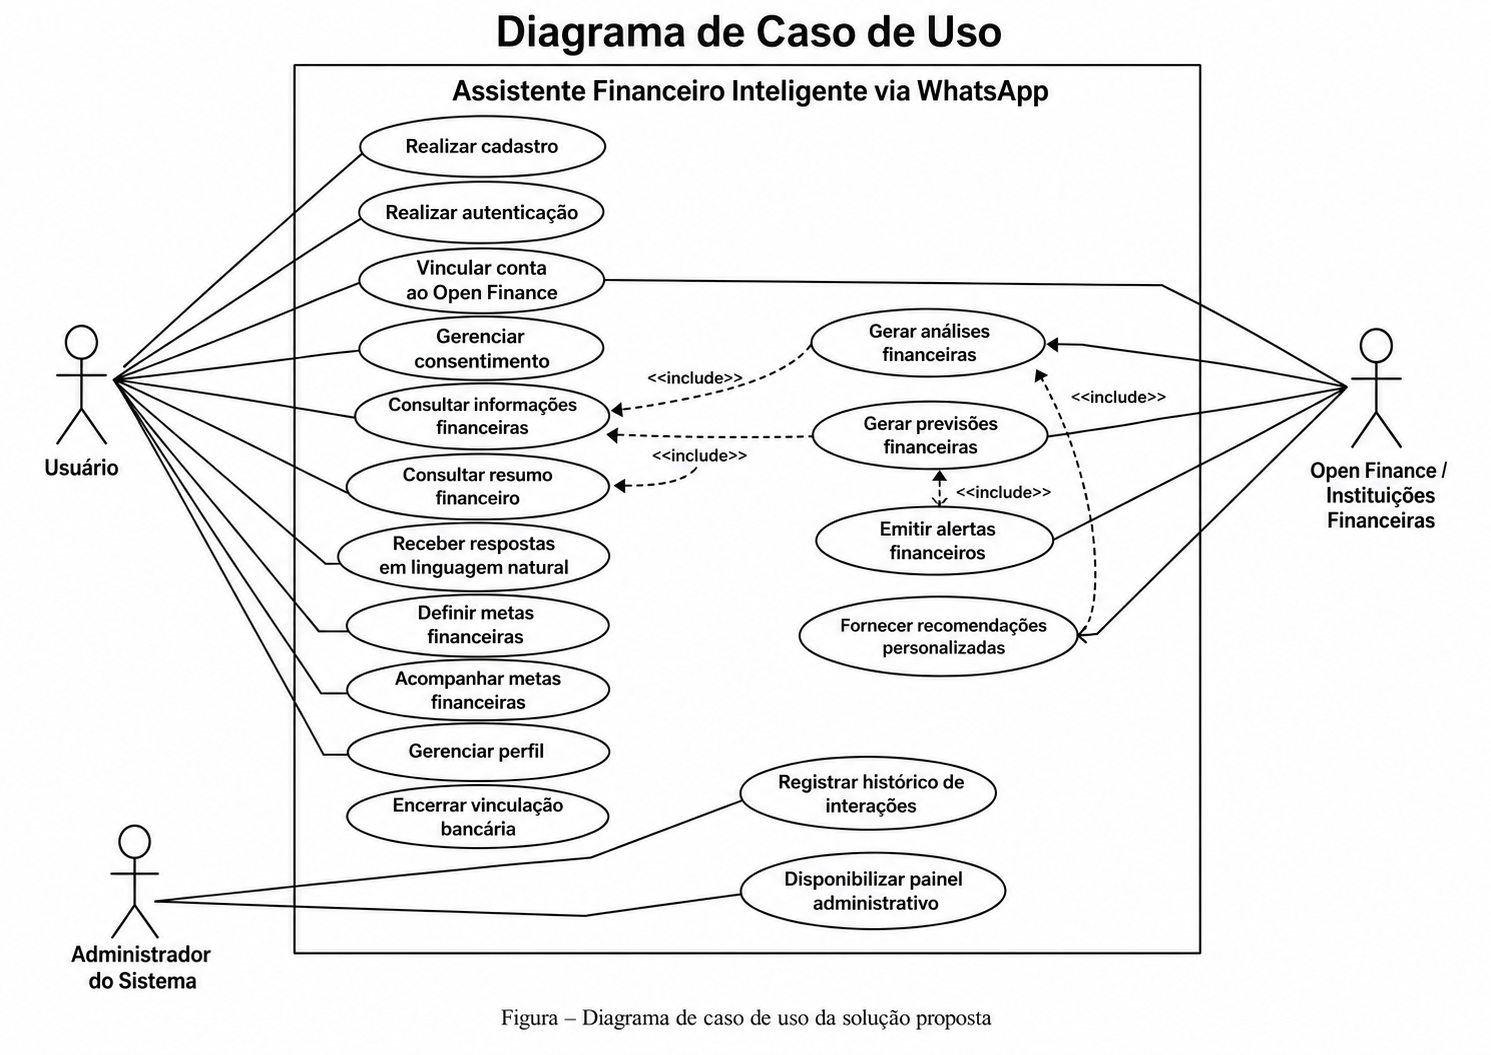
\includegraphics[width=1\textwidth]{images/uml.png}
    \fontetabela{\textbf{Fonte:} Elaborado pelos autores (2026).}
\end{figure}

\subsection{Descrição de casos de uso}

% A ser preenchido
